\documentclass{article}
\setlength{\parskip}{5pt} % esp. entre parrafos
\setlength{\parindent}{0pt} % esp. al inicio de un parrafo
\usepackage{amsmath} % mates
\usepackage[sort&compress,numbers]{natbib} % referencias
\usepackage{url} % que las URLs se vean lindos
\usepackage[top=25mm,left=20mm,right=20mm,bottom=25mm]{geometry} % margenes
\usepackage{hyperref} % ligas de URLs
\usepackage{graphicx} % poner figuras
\usepackage[spanish]{babel} % otros idiomas

\author{Raul Lagunes Rivera} % author
\title{Tarea P0 } % titulo
\date{\today}
\begin{document} % inicia contenido

\maketitle % cabecera

\begin{abstract} % resumen
  Es simplemente una demo sencilla del uso b\'{a}sico de \LaTeX{} en
  Overleaf.
\end{abstract}

\section{Introducci\'{o}n}\label{intro} % seccion y etiqueta



Este es un texto ejemplo para que hagan los reportes de sus
tareas. Vamos a incluir una ecuaci\'{o}n \eqref{equ}:
\begin{equation}
  f(x) = 2 \sin(x) - \int_0^\infty \frac{1}{1 + x} \text{d}x.
  \label{equ}
\end{equation}

\begin{figure} % figura
    \centering
    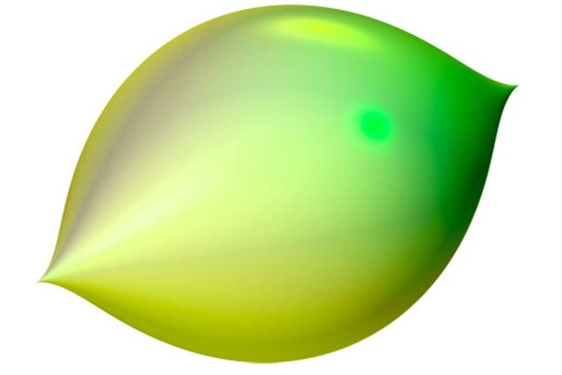
\includegraphics[width=60mm]{imagenes/limon.jpeg} % imagenes
     
    \caption{Lim\'{o}n tomado de \url{https://www.elmundo.es/elmundo/2011/01/25/ciencia/1295977576.html} con licencia CC.}
    \label{limon}
\end{figure}

\newpage

Vamos a aprender además a citar fuentes \citep{ejemplo}. Incluimos un cuadro \ref{datos} con algunos datos y en la figura \ref{limon} hay un limón.
 \begin{table}[h]
     \caption{Ocupo explicar de qué se trata mi cuadro.}
     \label{datos}
     \centering
     \begin{tabular}{|l|c|r|}
     \hline
          Algo & $\beta$ & $10.220$ \\
          \hline
          Otro & $\alpha$ & $1932.323$\\
          \hline
     \end{tabular}
 \end{table}
\vspace{2cm}
 \begin{figure}[h]
     \centering
     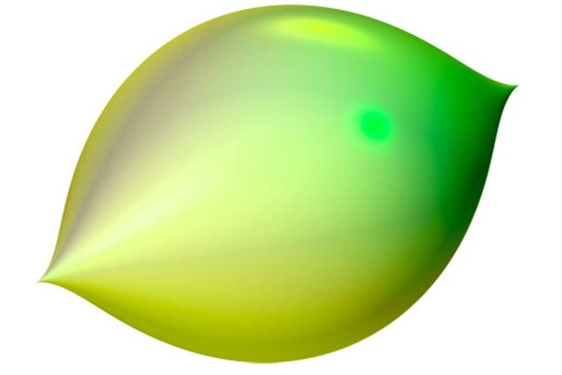
\includegraphics[width=60mm]{imagenes/limon.jpeg}
     \caption{Limón tomado de \url{https://www.elmundo.es/elmundo/2011/01/25/ciencia/1295977576.html} con licencia CC.}
     \label{limon}
 \end{figure}

 \section{Conclusiones}

 En este documento no más se hizo una intro en la sección \ref{intro} y luego ya se me quitaron las ganas de meterle más rollo.

 \bibliography{name.bib}
 \bibliographystyle{plainnat}

 \end{document}

